\section{Framework Design}

\section*{Um was geht es?}
\begin{itemize}
  \item Ein Framework ist ein Programmiergerüst, das dem Anwendungsprogramm einen Rahmen gibt und wiederverwendbare Funktionalität zur Verfügung stellt.
  \item Es bietet gezielt Orte an, wo es erweitert oder angepasst werden kann.
  \item In Frameworks kommen gewisse Design Patterns zum Einsatz.
  \item Frameworks werden heutzutage sehr häufig eingesetzt.
\end{itemize}

\section*{Lernziele LE 13 - Framework Design}
\begin{itemize}
  \item Sie sind in der Lage:
  \item die Eigenschaften von Frameworks zu nennen,
  \item Design Patterns im Einsatz von Frameworks anzuwenden,
  \item Prinzipen von modernen Frameworks zu verstehen,
  \item die Auswahl und den Gebrauch von Frameworks kritisch einzuschätzen.
\end{itemize}

\section*{1. Einleitung und Definition}
\begin{enumerate}
  \setcounter{enumi}{1}
  \item Design Patterns in Frameworks
  \item Fallstudie Persistenz-Framework
  \item Moderne Framework Patterns
  \item Wrap-up und Ausblick
\end{enumerate}

\section*{Framework Charakterisierung}
\begin{itemize}
  \item Leider gibt es keine allgemein akzeptierte exakte Definition eines Frameworks und der Begriff wird für viele Programmbibliotheken eingesetzt.
  \item Für unsere Zwecke möchten wir den Begriff folgendermassen abgrenzen:
  \item Ein Framework enthält keinen applikationsspezifischen Code.
  \item Ein Framework gibt aber den Rahmen («Frame») des anwendungsspezifischen Codes vor.
  \item Die Klassen eines Frameworks arbeiten eng zusammen, dies im Gegensatz zu einer reinen Klassenbibliothek wie z.B. die Java Collection Klassen.
  \item Ein Framework muss für den Einsatz gezielt erweitert und/oder angepasst werden.
  \item Applikations-Container wie z.B. Spring Framework oder Java EE (neu Jakarta EE) schliessen wir ebenfalls ein.
  \item Die Entwicklung eines neuen Frameworks ist eine aufwändige Angelegenheit.
  \item Wiederverwendbare Software (und dazu gehören natürlich Frameworks) sollte ein höheres Level im Bereich Zuverlässigkeit besitzen, was ebenfalls mit zusätzlichem Aufwand verbundenen ist.
  \item Erweiterbare Software (und dazu gehören natürlich Frameworks) erfordert eine tiefergehende Analyse darüber, welche Teile erweiterbar sein sollen, was zu einem höheren Architektur- und Designaufwand führt.
  \item Eigentlich sprechen alle diese Punkte dagegen, selber ein Framework zu entwickeln. Weshalb wird dies trotzdem behandelt?
\end{itemize}

\section*{Framework Einsatz und Entwicklung erweiterbarer Software}
\begin{itemize}
  \item Alle Design Patterns, die wir heute behandeln, können für die Entwicklung erweiterbarer Software eingesetzt werden.
  \item Dies muss nicht zwingend ein Framework sein, das auf GitHub publiziert wird, sondern es kann auch einfach eine Komponente sein, die in mehreren eigenen Anwendungen in verschiedenen Kontexten eingesetzt wird.
  \item Das Wissen um den Aufbau von Frameworks hilft auch, deren Einsatz, aber auch deren Grenzen zu verstehen.
\end{itemize}

\section*{Kritische Bemerkungen zu Frameworks}
\begin{itemize}
  \item Frameworks tendieren dazu, im Laufe der Zeit immer mehr Funktionalität zu «sammeln».
  \item Was auf den ersten Blick positiv scheint, kann im zweiten Blick zu inkonsistentem Design und funktionalen Überschneidungen führen, die den Einsatz immer mehr erschweren.
  \item Der Einsatz eines Frameworks sollte gut überlegt werden.
  \item Einerseits erfordert dies gute Kenntnisse des Frameworks, andererseits ist nach der «Verheiratung» der Anwendung mit dem Framework eine «Scheidung» nur noch schwierig und mit hohem Aufwand möglich.
  \item Allenfalls sollte das Framework nur über eigene Schnittstellen verwendet werden (keine direkte Abhängigkeit), was aber unter Umständen die Nützlichkeit des Einsatzes in Frage stellt.
\end{itemize}

\begin{enumerate}
  \item Einleitung und Definition
  \item Design Patterns in Frameworks
  \item Fallstudie Persistenz-Framework
  \item Moderne Framework Patterns
  \item Wrap-up und Ausblick
\end{enumerate}

\section*{Recap: Aufbau Design Patterns}
\begin{itemize}
  \item Beschreibungsschema
  \item Name
  \item Beschreibung Problem
  \item Beschreibung Lösung
  \item Hinweise für Anwendung
  \item Beispiele
\end{itemize}

\section*{Recap: Anwendung von Design Patterns}
\begin{itemize}
  \item Design Patterns sind ein wertvolles Werkzeug, um bewährte Lösungen für wiederkehrende Probleme schnell zu finden.
  \item Sie helfen, im Team effizient über Lösungsmöglichkeiten zu kommunizieren.
  \item Ihre Anwendung stellt aber immer einen Trade-Off zwischen Flexibilität und Komplexität dar.
  \item Es ist keineswegs so, dass ein Programm automatisch besser wird, wenn mehr Patterns angewendet werden.
\end{itemize}

\section*{Design Patterns}
\begin{itemize}
  \item Abstract Factory
  \item Factory Method
  \item Command
  \item Template Method
\end{itemize}

\section*{Abstract Factory: Problem und Lösung}
\section*{- Problem}
\begin{itemize}
  \item Die Erzeugung verschiedener, inhaltlich zusammengehörender Objekte («Product»), ohne aber die konkreten Klassen zu kennen, damit diese austauschbar sind.
  \item Lösung
  \item Eine AbstractFactory und abstrakte «Products» definieren.
  \item Die AbstractFactory hat für jedes «Product» eine eigene «create» Methode.
  \item Eine konkrete Factory davon ableiten, die dann konkrete «Products» erzeugt.\\
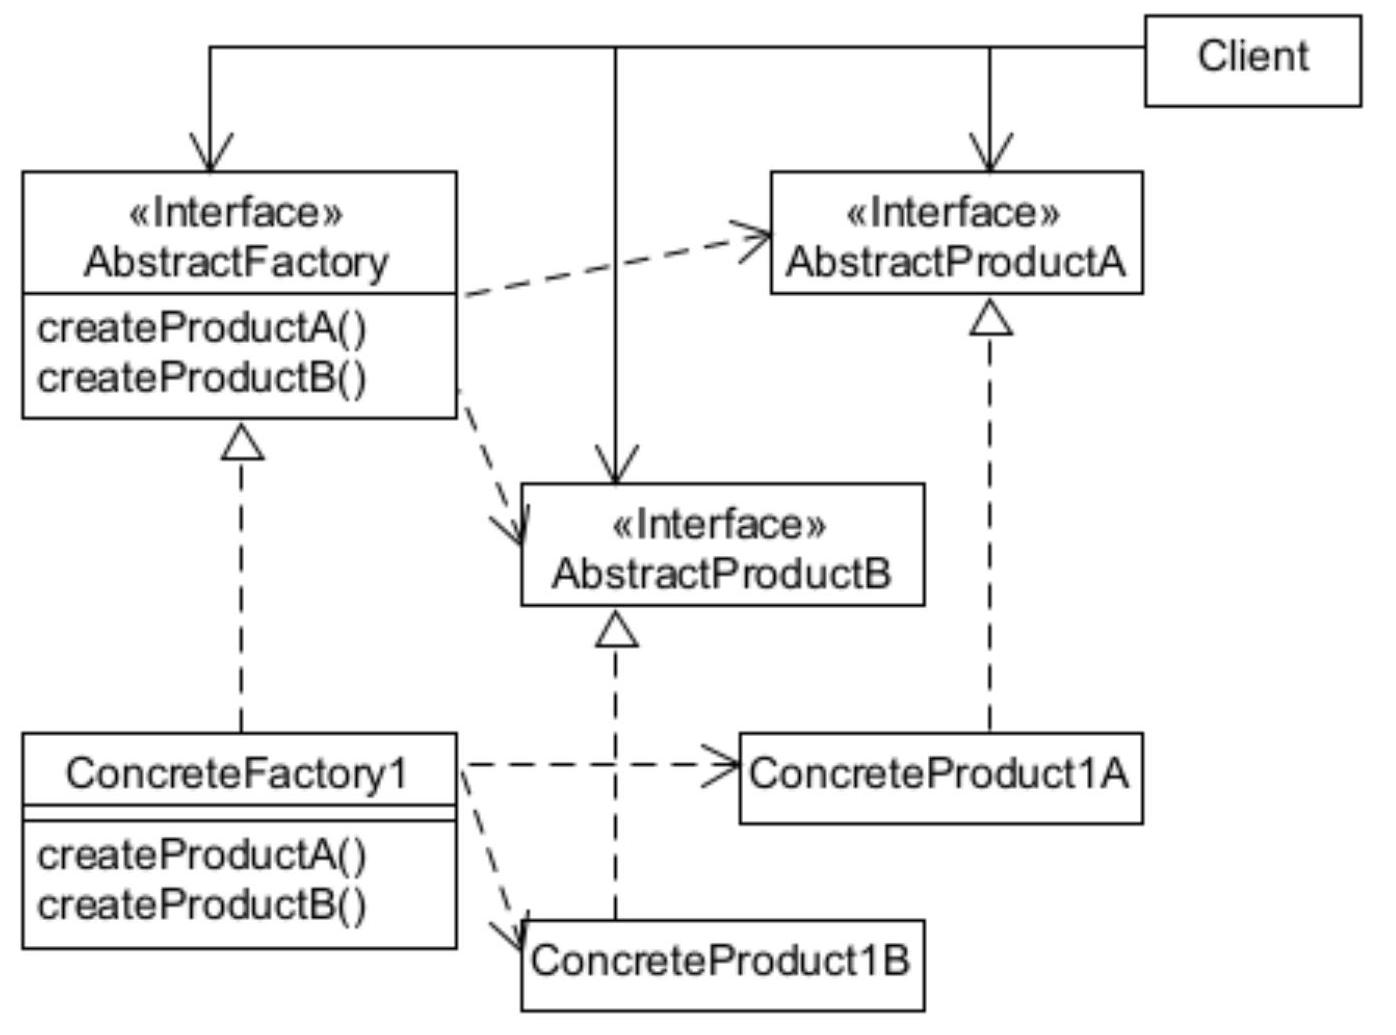
\includegraphics[max width=\textwidth, center]{2025_01_02_73d93f10fa91ab6123dcg-13}
\end{itemize}

\section*{Abstract Factory: Hinweise}
\begin{itemize}
  \item Hinweise
  \item Eigentlich «nur» eine Verallgemeinerung einer «SimpleFactory».
  \item Die verschiedenen Produkte hängen inhaltlich miteinander zusammen, zum Beispiel verschiedene Teile der anzusteuernden Hardware.\\
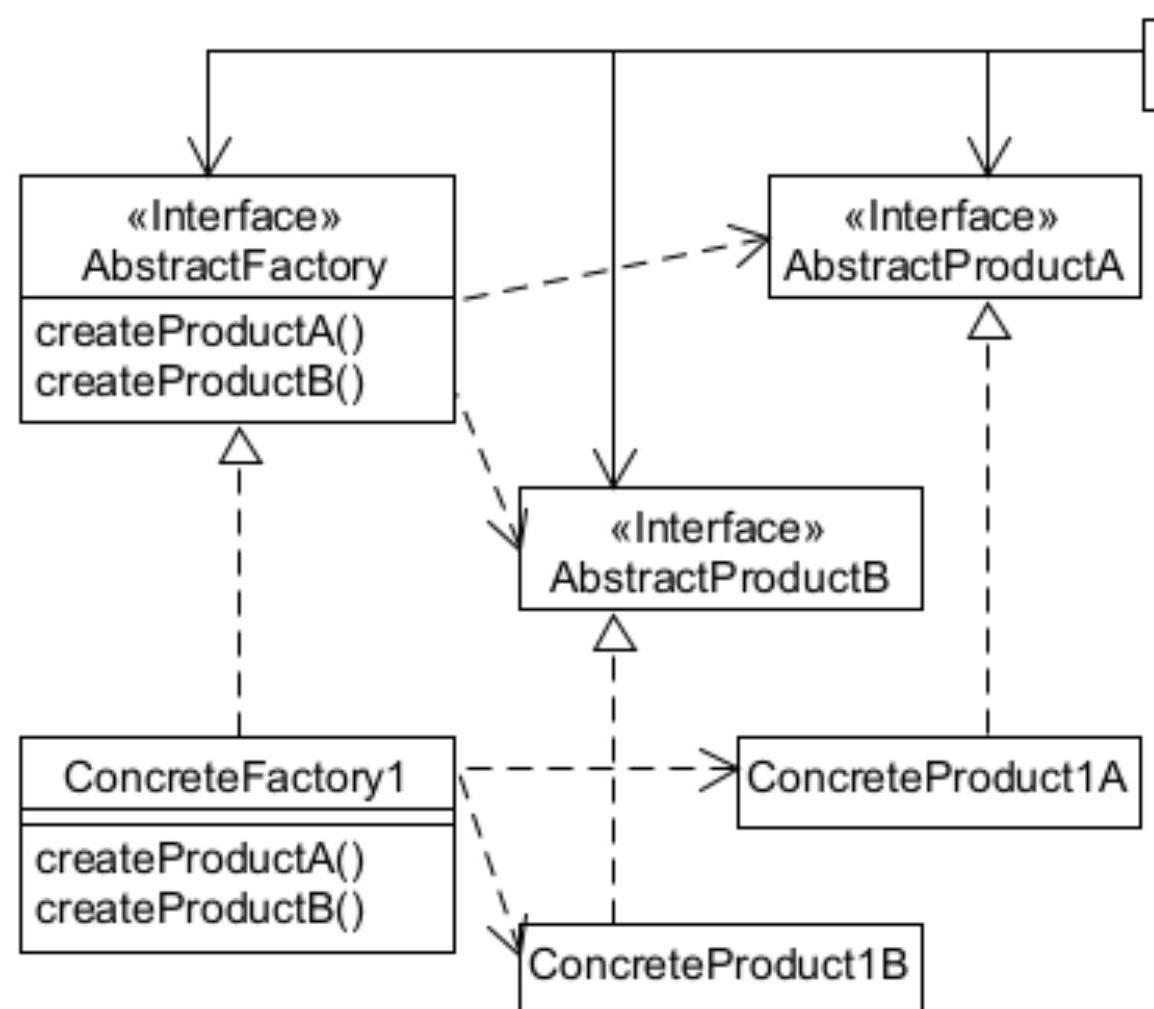
\includegraphics[max width=\textwidth, center]{2025_01_02_73d93f10fa91ab6123dcg-14}
\end{itemize}

\section*{Abstract Factory: Beispiel Point Of Sale (POS) Terminal}
School of Engineering

\begin{itemize}
  \item Die elektronische Kasse muss Hardware wie z.B. die Notenschublade oder den Münzspender ansteuern.
  \item Typischerweise kommen die einzelnen Komponenten vom selben Hersteller.
  \item Pro Hersteller gibt es eine konkrete Implementation von IJavaPOSDevicesFactory.
\end{itemize}

\begin{verbatim}
this is the Abstract
this is the Abstract 
Factory--an interface fo
creating a family of
related objects
\end{verbatim}

\begin{center}
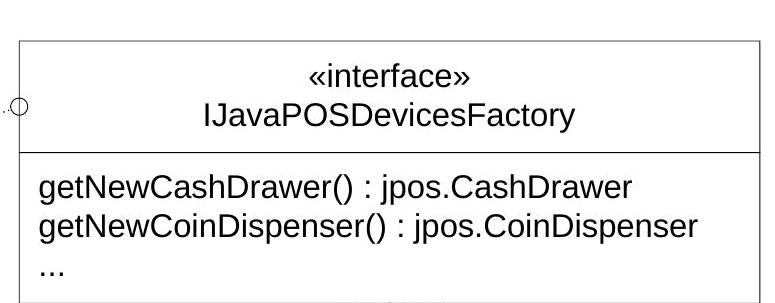
\includegraphics[max width=\textwidth]{2025_01_02_73d93f10fa91ab6123dcg-15}
\end{center}

Abstract Factory $\swarrow$

Konkrete Factory\\
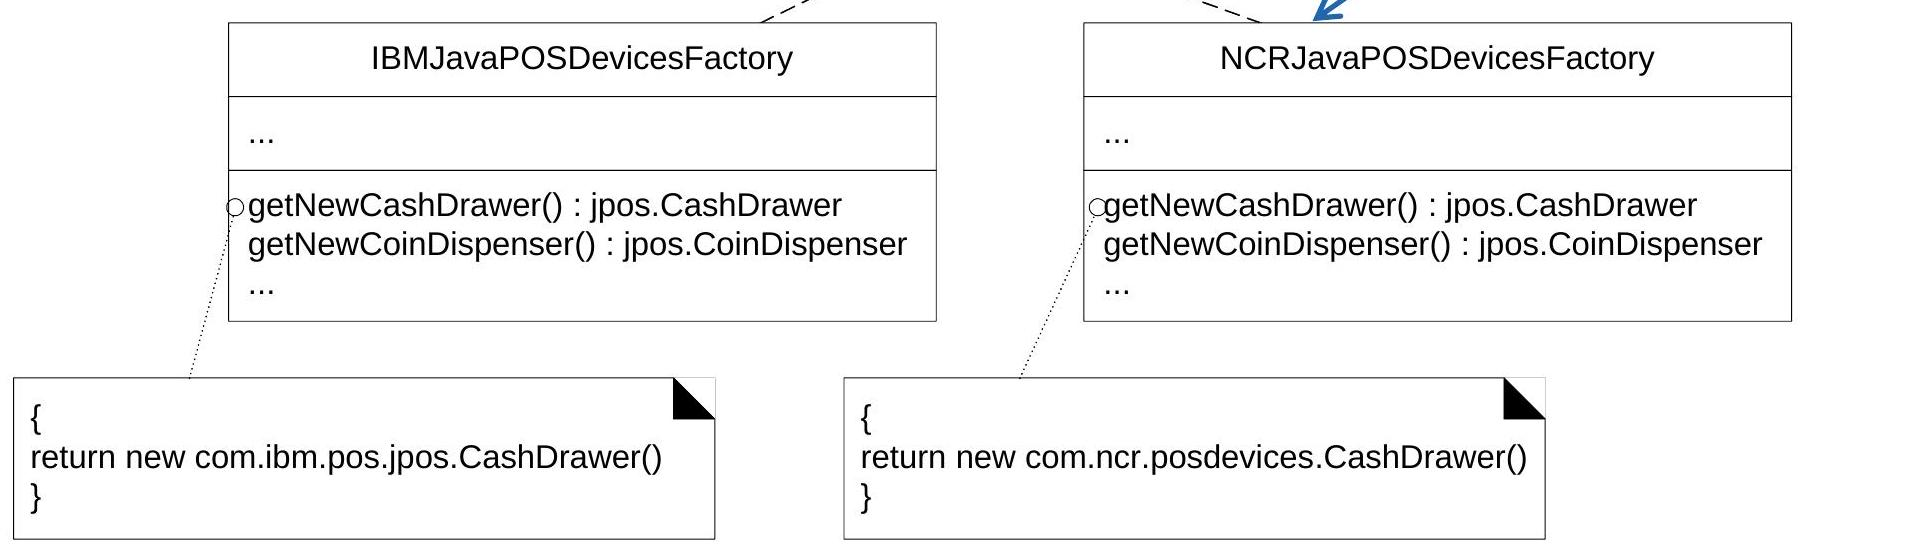
\includegraphics[max width=\textwidth, center]{2025_01_02_73d93f10fa91ab6123dcg-15(1)}\\
com.ncr.posdevices.CashDrawer\\
isDrawerOpened()

\section*{Factory Method: Problem und Lösung}
\begin{itemize}
  \item Problem
  \item Eine (wiederverwendbare) Klasse Creator hat die Verantwortlichkeit, eine Instanz der Klasse Product zu erzeugen. Es ist aber klar, dass Product noch spezialisiert werden muss.
  \item Lösung
  \item Eine abstrakte Methode in der Klasse Creator definieren, die als Resultat Product zurückliefert.
  \item Konkrete Klassen von Creator können dann die\\
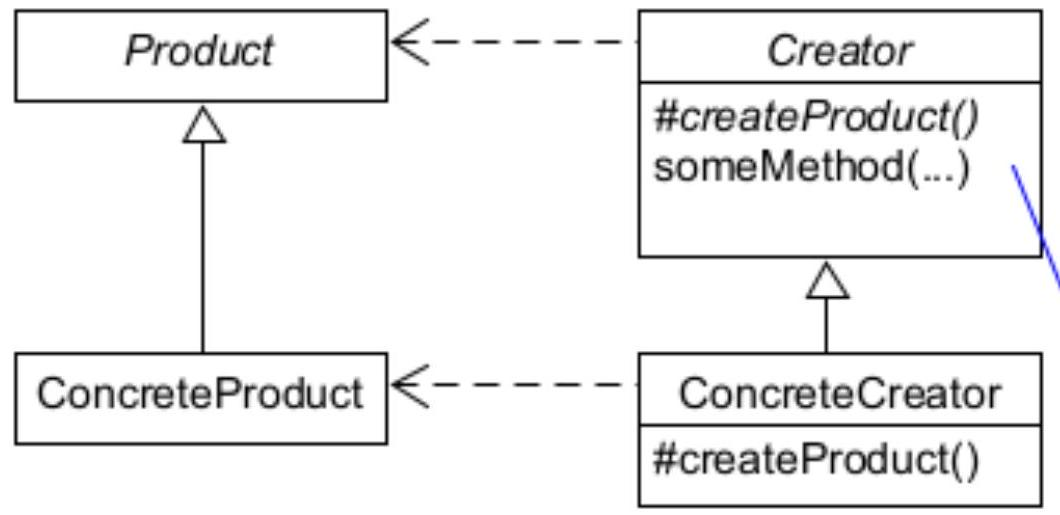
\includegraphics[max width=\textwidth]{2025_01_02_73d93f10fa91ab6123dcg-16} richtige Subklasse von Product erzeugen.
\end{itemize}

\section*{Factory Method: Hinweise}
\begin{itemize}
  \item Hinweise
  \item Es ist durchaus erlaubt, dass bereits Creator und Produkt konkret sind und somit eine Basisfunktionalität zur Verfügung stellen.
  \item Es gibt parallele Vererbungshierarchien mit Creator wie auch Product an der Spitze.
  \item Kann auch als Variante des Design Patterns «Template Method» interpretiert werden.\\
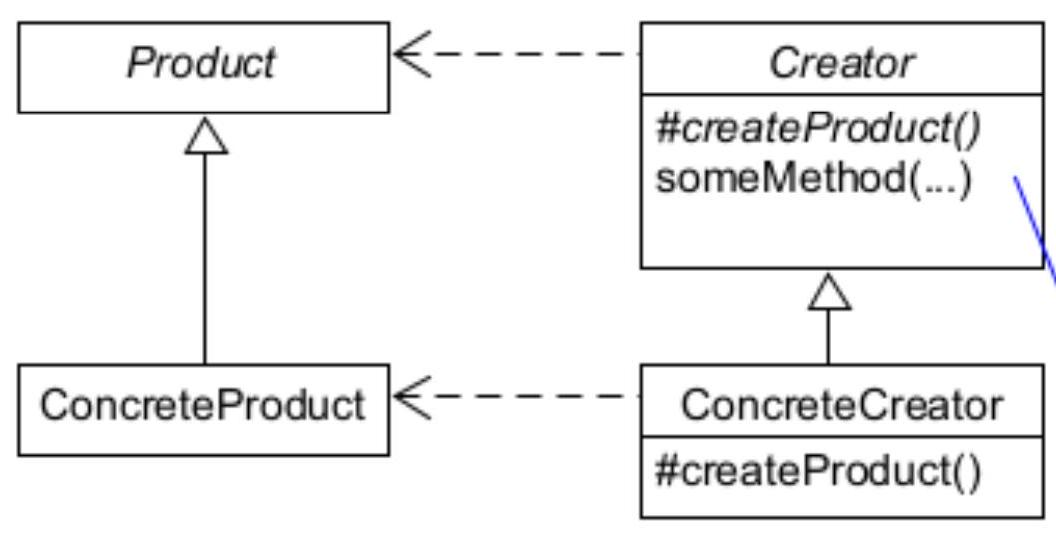
\includegraphics[max width=\textwidth, center]{2025_01_02_73d93f10fa91ab6123dcg-17}
\end{itemize}

\section*{Factory Method: Beispiel GoF (2/2)}
\begin{itemize}
  \item Das Zeichenprogramm («Client») besitzt eine KlassenHierarchie von Figuren.
  \item Um Figuren übers UI verändern zu können, gibt es eine abstrakte Manipulator Klasse.
  \item Jede konkrete Figur hat nun die Aufgabe, seine Manipulator Klasse zu instanziieren.\\
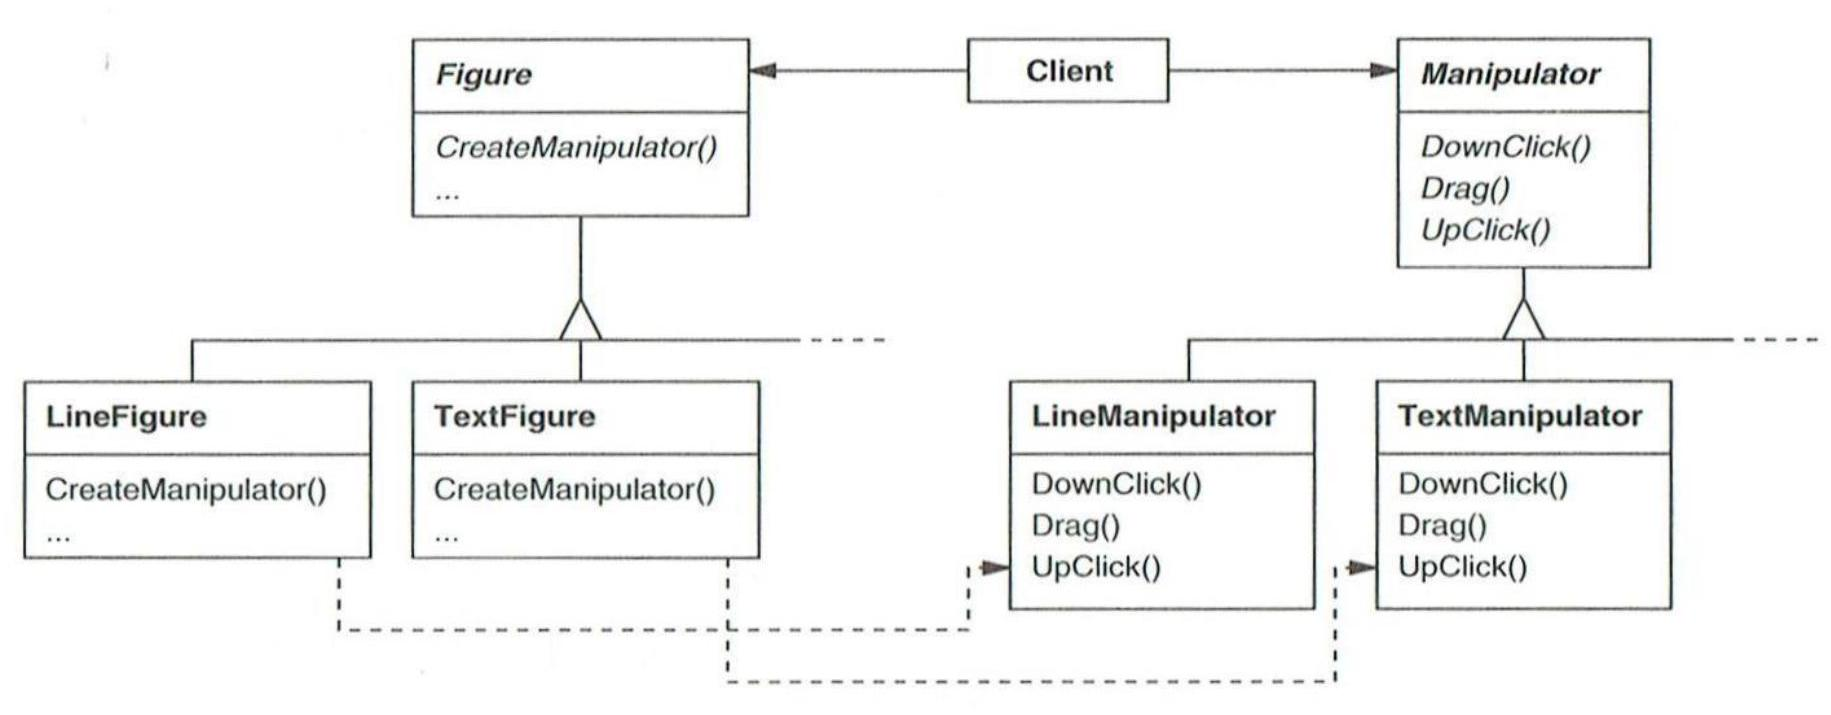
\includegraphics[max width=\textwidth, center]{2025_01_02_73d93f10fa91ab6123dcg-18}
\end{itemize}

\section*{Command: Problem und Lösung}
\begin{itemize}
  \item Problem
  \item Aktionen müssen für einen späteren Gebrauch gespeichert werden und dabei können sie noch allenfalls priorisiert oder protokolliert werden und/oder Unterstützung für ein Undo anbieten.
  \item Lösung
  \item Ein Interface wird definiert, das nur die Auslösung der Aktion erlaubt.
  \item Implementationen dieses Interface überschreiben die Methode zur Auslösung der Aktion.
  \item Meistens bedeutet die Aktion, dass eine Methode auf\\
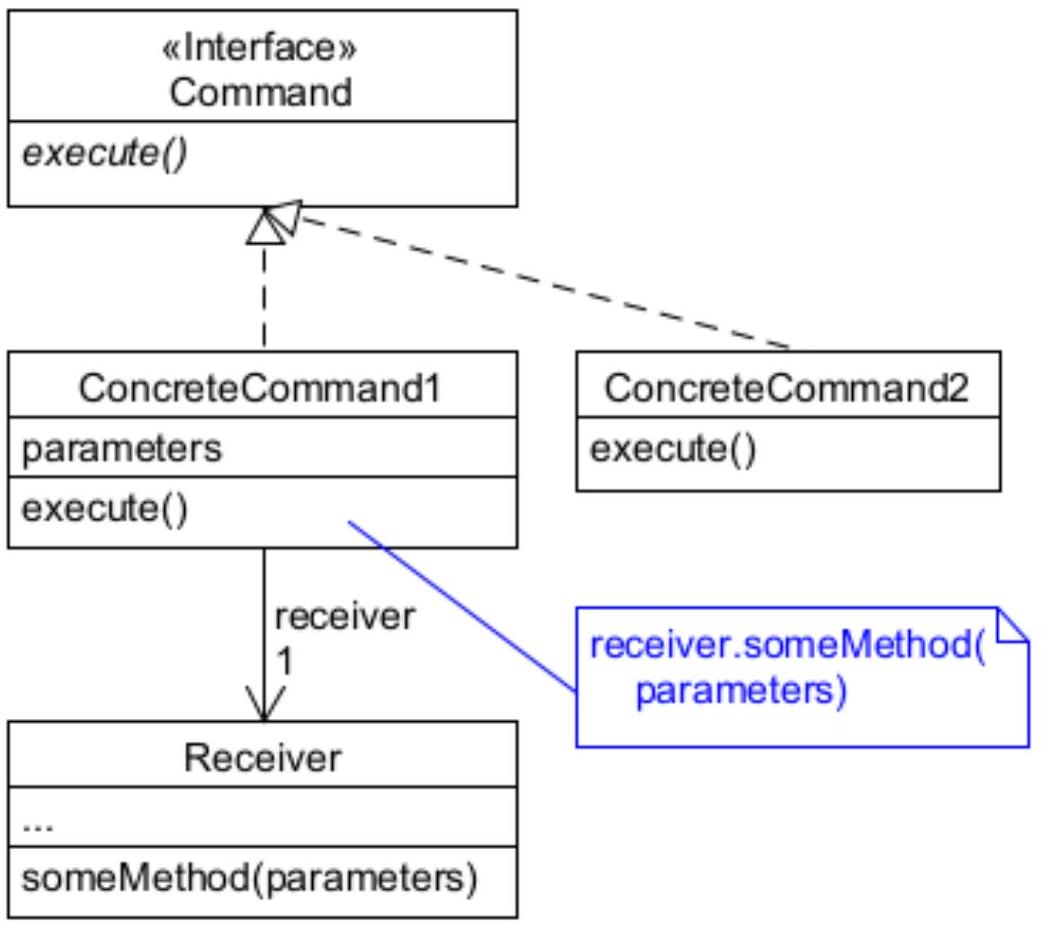
\includegraphics[max width=\textwidth]{2025_01_02_73d93f10fa91ab6123dcg-19} einem anderen Objekt aufgerufen wird.
  \item Dazu muss die Aktion die Parameter dieser Methode zwischenspeichern.
\end{itemize}

\section*{Command: Hinweise}
\begin{itemize}
  \item Hinweise
  \item Erstellung der Aktion und das Auslösen liegen zeitlich auseinander.
  \item Bevor Aktionen ausgelöst werden, können sie bei Bedarf noch sortiert oder priorisiert werden. Denken Sie dabei an eine Datenbank.
  \item Der Receiver muss nicht zwingend über eine Assoziation sichtbar sein. Es ist auch ein Lookup über z.B. einen Namen denkbar.
  \item Falls eine Rückabwicklung der Aktion («Undo») notwendig ist, kann die entsprechende Methode direkt in der Aktion eingefügt werden oder es gibt eine separate Aktion dafür.\\
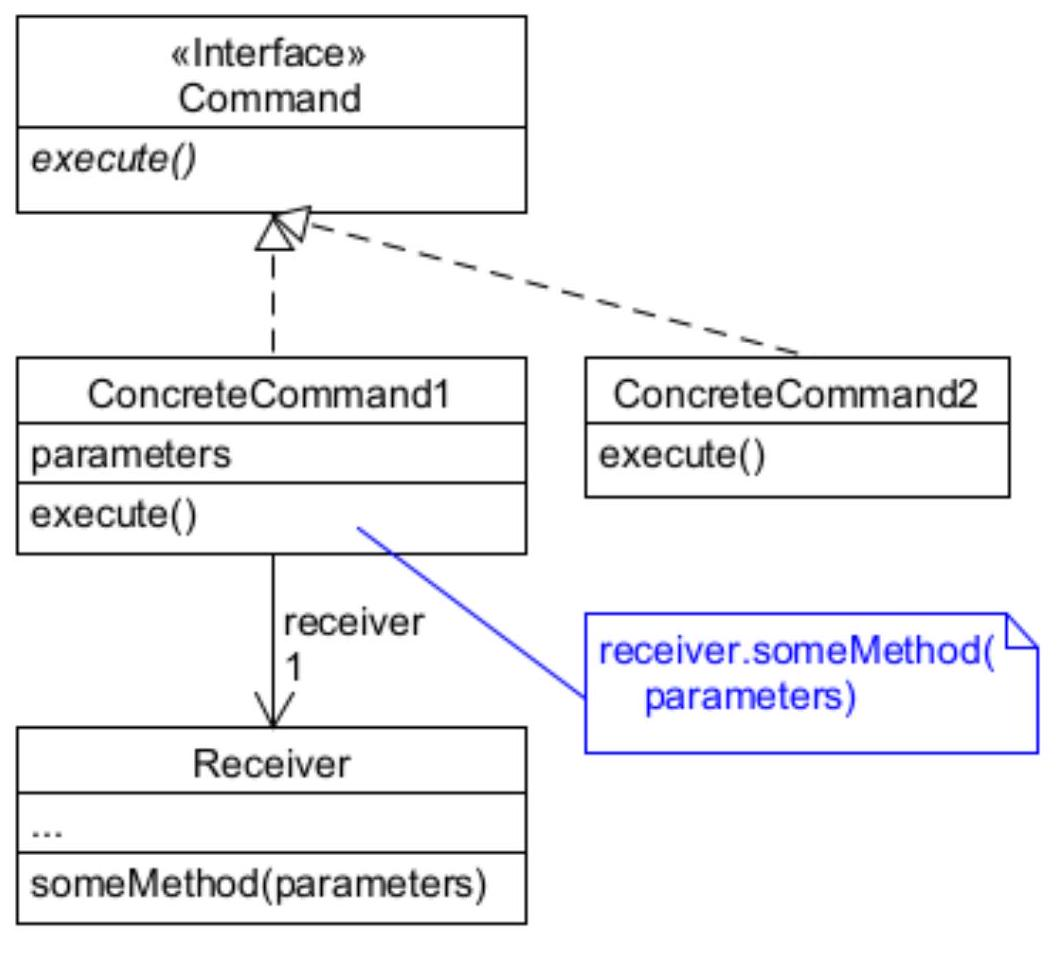
\includegraphics[max width=\textwidth, center]{2025_01_02_73d93f10fa91ab6123dcg-20}
\end{itemize}

\section*{Command: Beispiel Point Of Sale Terminal}
\begin{itemize}
  \item Eine Transaktion eines Persistenz-Frameworks setzt sich aus den Aktionen für jedes veränderte Objekt zusammen.
  \item Aktionen sind update, insert und delete.
  \item Eine undo Methode ist ebenfalls vorhanden.\\
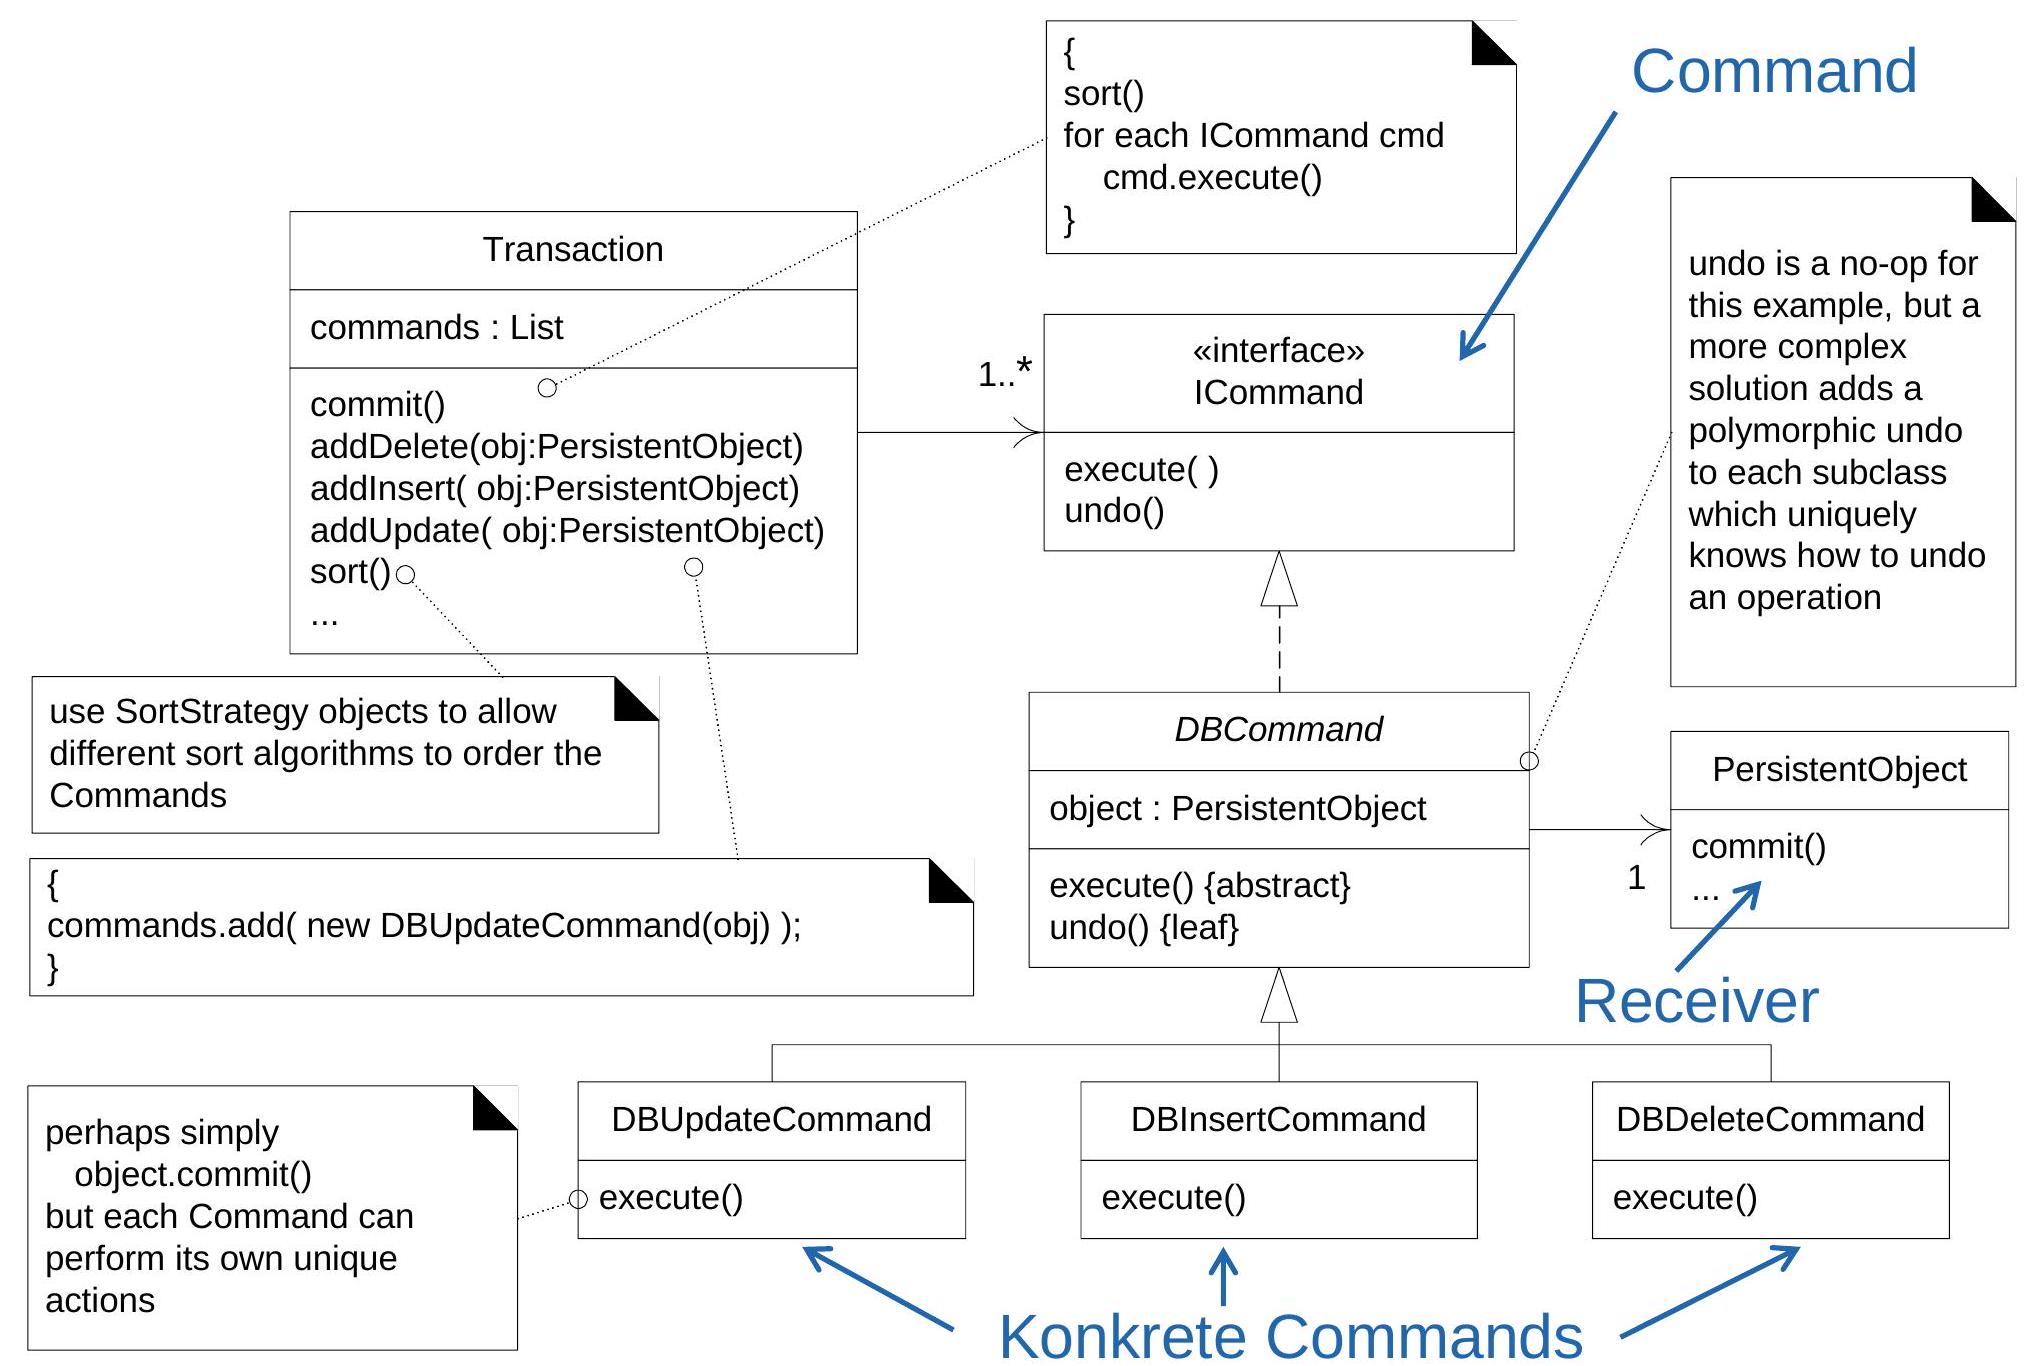
\includegraphics[max width=\textwidth, center]{2025_01_02_73d93f10fa91ab6123dcg-21}
\end{itemize}

\section*{Template Method: Problem und Lösung}
\begin{itemize}
  \item Problem
  \item Ein Ablauf/Algorithmus soll so entworfen werden, dass er in gewissen Punkten angepasst werden kann.
  \item Lösung
  \item In einer abstrakten Klasse wird eine Template Method hinzugefügt, die diesen Ablauf/Algorithmus implementiert.
  \item Die Template Method ist fertig geschrieben, ruft aber noch abstrakte Methoden («hookMethod») auf.
  \item Diese Methoden dienen als Variations- resp. Erweiterungspunkte\\
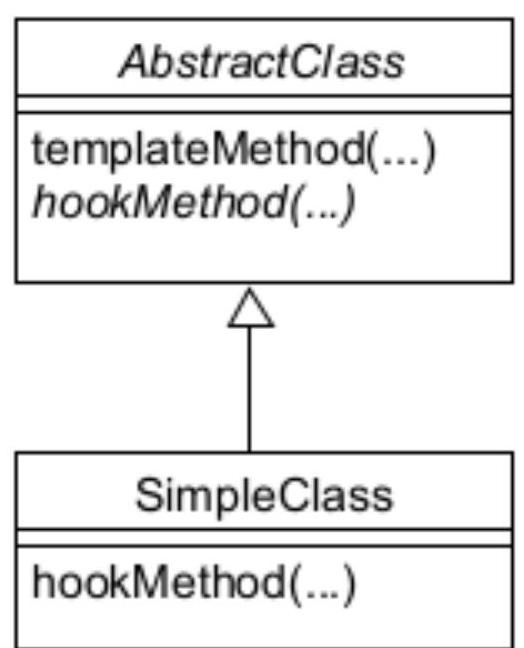
\includegraphics[max width=\textwidth]{2025_01_02_73d93f10fa91ab6123dcg-22} und mit ihrer Implementation kann der Ablauf/Algorithmus auf den aktuellen Kontext angepasst werden.
\end{itemize}

\section*{Template Method: Hinweise}
\begin{itemize}
  \item Hinweise
  \item Die «hookMethod» kann entweder rein abstrakt sein oder bereits eine Standard-Implementation enthalten.
  \item Eine Factory Method kann in diesem Zusammenhang ebenfalls als «hookMethod» interpretiert werden.
  \item Es ist nicht einfach, im Voraus alle Orte zu identifizieren, wo Anpassungen notwendig sein müssen.
  \item Verwandtschaft mit einer Strategy. Eine Strategy benutzt Delegation, um einen ganzen Algorithmus zu variieren, während\\
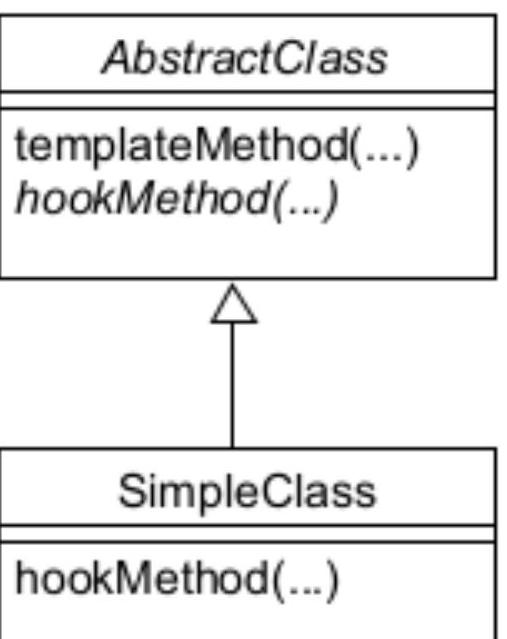
\includegraphics[max width=\textwidth]{2025_01_02_73d93f10fa91ab6123dcg-23} Template Method Vererbung benutzt, um einen Teil des Algorithmus zu variieren.
  \item Hollywood Prinzip: «Don’t call us, we call you». Der eigene Code wird von fremdem Code aufgerufen (oder: der Code des Frameworks ruft den Code der Umsetzung auf).
\end{itemize}

\section*{Template Method: Beispiel Larman GUI Framework}
School of Engineering\\
InIT Institut für angewandte Informationstechnologie

\section*{- Ein GUI Framework stellt Komponenten zur Verfügung.}
\begin{itemize}
  \item Die Basisklasse GUIComponent stellt die Template Method update() zur Verfügung, die repaint() aufruft.
  \item Die Methode repaint() muss dann von unserer Klasse überschrieben werden.\\
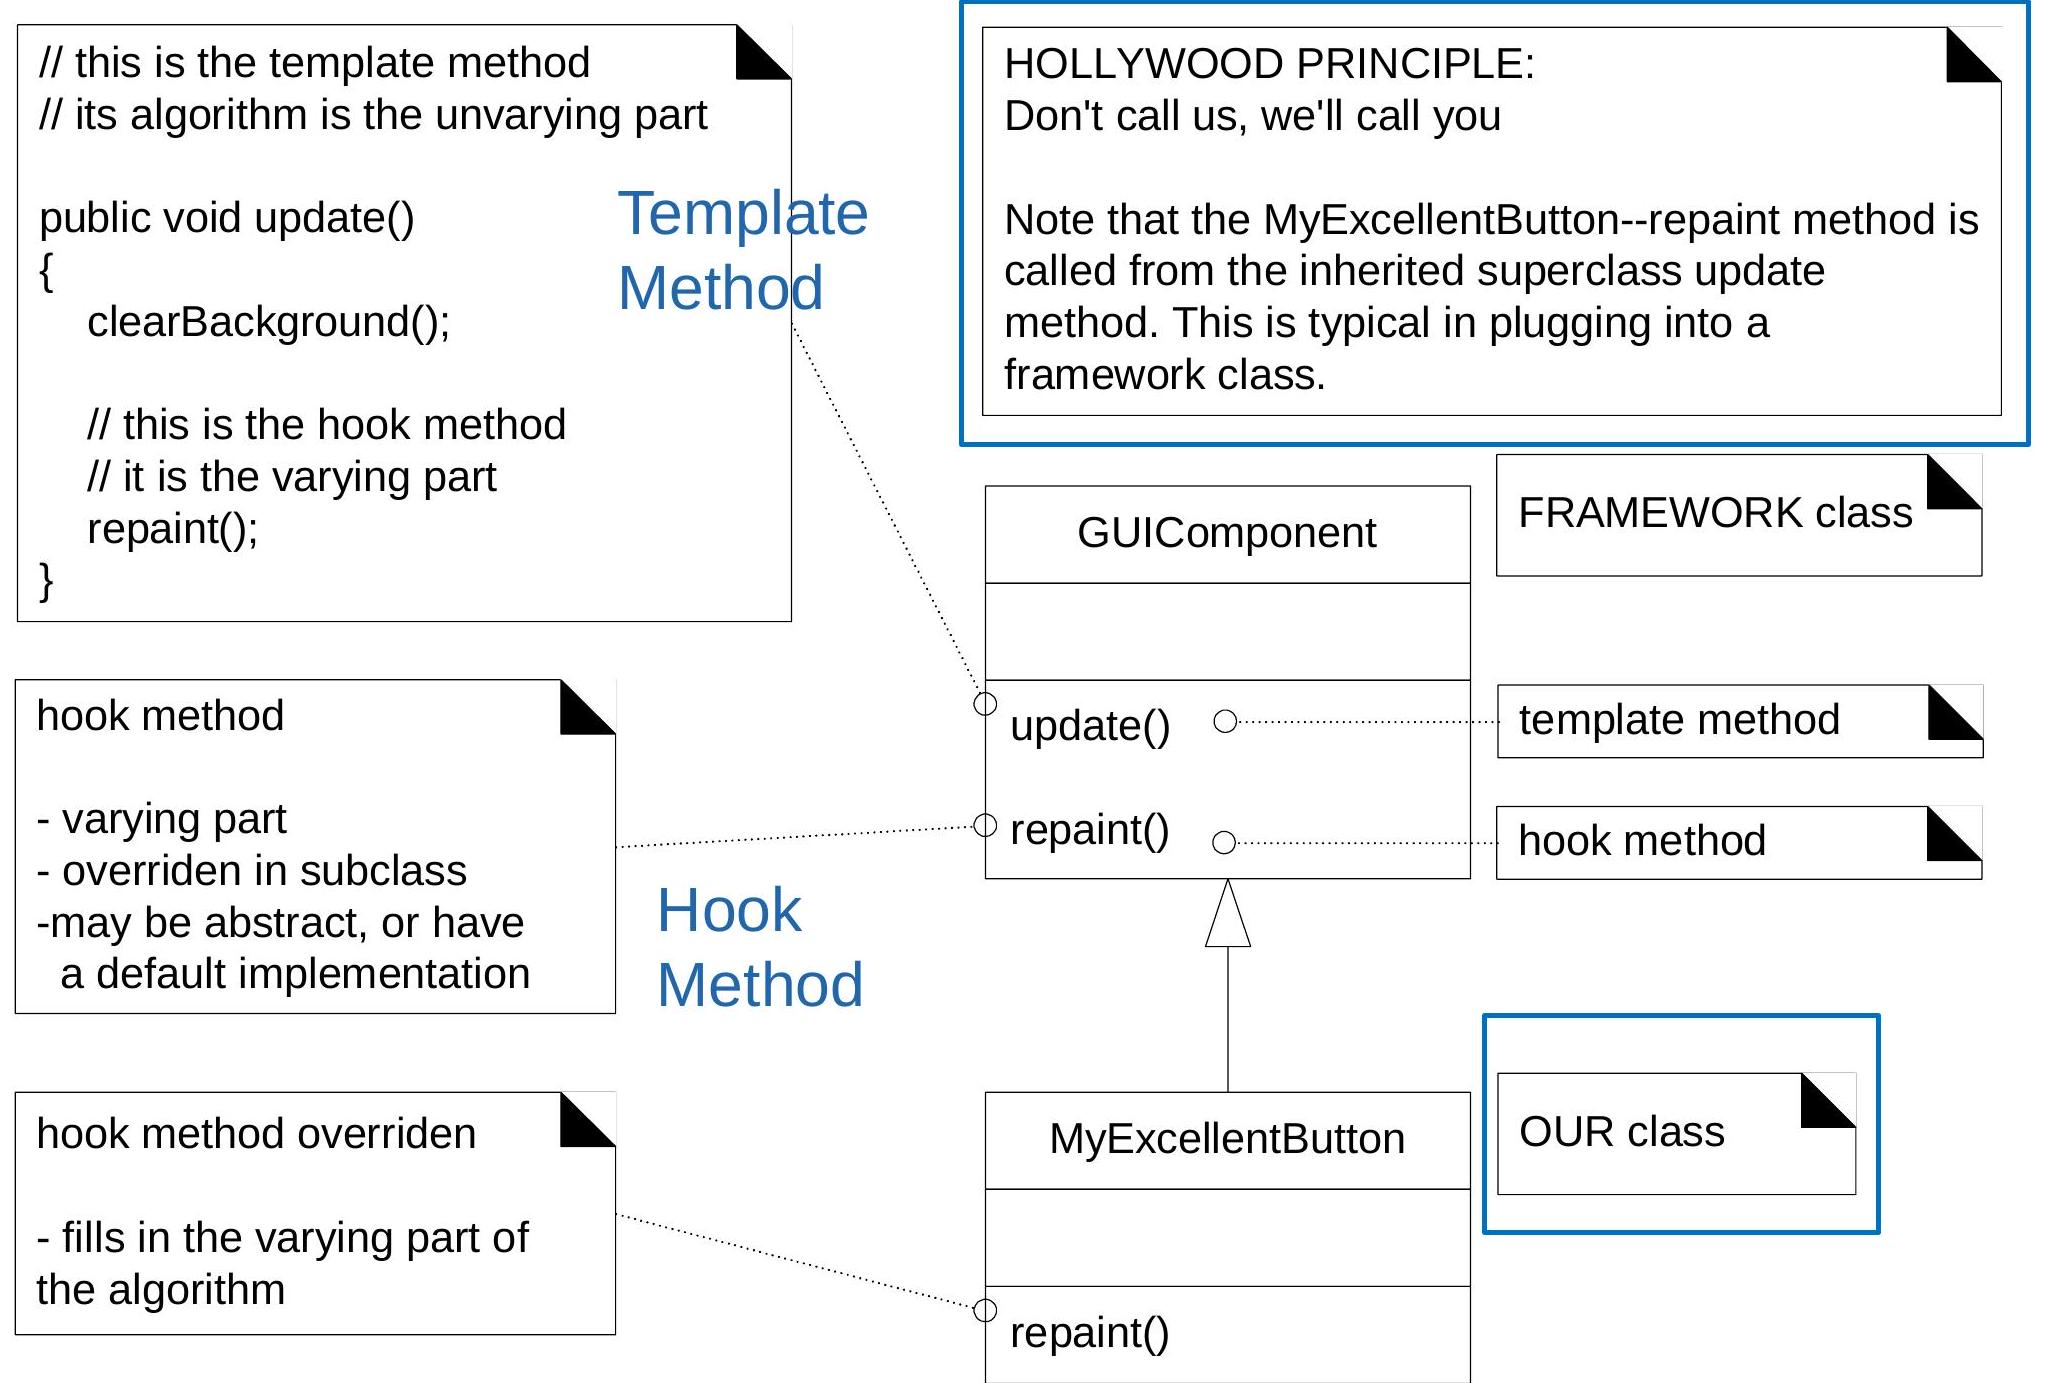
\includegraphics[max width=\textwidth, center]{2025_01_02_73d93f10fa91ab6123dcg-24}
\end{itemize}

\begin{enumerate}
  \item Einleitung und Definition
  \item Design Patterns in Frameworks
  \item Fallstudie Persistenz-Framework
  \item Moderne Framework Patterns
  \item Wrap-up und Ausblick
\end{enumerate}

\section*{Einleitung Persistenz-Framework im Buch von Larman}
\begin{itemize}
  \item Framework für Speicherung von Objekten (siehe [1] Kap. 38).
  \item Primäres Ziel: Prinzipien des Framework Designs zeigen.
  \item Sekundäres Ziel: Problemstellungen von Persistenz-Frameworks und mögliche Lösungsansätze zeigen.
  \item Was fehlt?
  \item Eigentliche RDB-Zugriffe. Im Buch werden verschiedene Lösungen skizziert.
  \item Eigentliche Behandlung von Collections und Assoziationen. Im Buch wird dafür die Verwendung vom Design Pattern «Virtual Proxy» erwähnt.
  \item Abfragen (Queries) werden gar nicht behandelt. Da ja beliebige Speichertechnologien unterstützt werden sollen, ist dies aber auch nicht verwunderlich.
  \item Der vollständige Programmcode.
\end{itemize}

\section*{Themen Persistenz-Framework von Larman}
\begin{itemize}
  \item Persistenz-Fassade
  \item Mapping auf RDB
  \item Mapper für jede Klasse
  \item Objekt-Identifikation
  \item Verfeinerung Mapper
  \item Zustandsverwaltung bezüglich Transaktionen
  \item Proxy für Lazy Loading von referenzierten Objekten
\end{itemize}

\begin{enumerate}
  \item Einleitung und Definition
  \item Design Patterns in Frameworks
  \item Fallstudie Persistenz-Framework
  \item Moderne Framework Patterns
  \item Wrap-up und Ausblick
\end{enumerate}

\section*{Moderne Framework Patterns}
\begin{itemize}
  \item Die bewährten Design Patterns finden nach wie vor ihre Anwendung im Framework Design.
  \item In den letzten Jahren wurden aber noch weitere Mechanismen populär.
  \item Dependency Injection, meistens gesteuert über Annotationen
  \item Convention over Configuration: Nur durch das Einhalten von (Namens-)Konventionen wird das Framework aktiv und macht das Gewünschte.
  \item Implementation von Interfaces basierend auf den Methoden des Interfaces (z.B. Spring Data Repository-Interfaces). Der Methodenname spezifiziert sozusagen seine Implementation, allenfalls noch ergänzt mit Annotationen
  \item Ist ein Standard Java-Sprachelement ab Java 5 (z.B. @override).
  \item Können selber deklariert werden.
  \item Werden «normalen» Sprachelementen hinzugefügt
  \item Vorteil: Wenn beim Laden einer annotierten Klasse die Annotations-Klasse nicht gefunden wird, gibt es keine Fehlermeldung, sondern die Annotation wird stillschweigend entfernt.
  \item Anders gesagt fügen Annotationen keine harte Abhängigkeit hinzu und sind somit geeignet, die Domänenlogik frei von ungewünschten (technischen) Abhängigkeiten zu halten.
\end{itemize}

\section*{Steuerung über Annotationen}
\begin{itemize}
  \item Annotationen per se haben ja keine Funktionalität. Es braucht «jemand», der die Annotationen liest und dann Aktionen ausführt.
  \item Auswertung von Annotationen:
  \item Beim Starten der Anwendung wird das Framework ebenfalls gestartet.
  \item Das Framework sucht die Anwendungsklassen auf dem Klassenpfad ab, untersucht allfällige Annotationen und führt die gewünschten Aktionen aus.
  \item Mögliche Aktionen des Frameworks:
  \item Dependency Injection von Framework Objekten in Anwendungsobjekte (über Constructor oder Set-Methode).
  \item Automatisches Implementieren von Interfaces.
  \item Hinzufügen von Funktionalität zu Anwendungsklassen.
  \item Achtung: Dieser Vorgang kann zu unerwünschten Verzögerungen beim Start führen.
\end{itemize}

\section*{Java Mechanismen für das Hinzufügen von Funktionalität}
\begin{itemize}
  \item 2 Zeitpunkte
  \item Während (respektive am Schluss) der Kompilierung über einen AnnotationProcessor.
  \item Beim Starten einer Anwendung können Anwendungsklassen beim Laden (über einen FrameworkClassloader) noch verändert werden.
  \item Was wird verändert
  \item Quellcode hinzufügen.
  \item Bytecode hinzufügen und bestehenden abändern.
  \item Für das Implementieren von Interfaces kann java.lang.reflect.Proxy eingesetzt werden.
  \item Wer verändert
  \item AnnotationProcessor kann Quellcode und Bytecode hinzufügen.
  \item Beim Starten einer Anwendung kann Byte Code verändert und hinzugefügt, sowie die Proxy Klasse angewendet werden.
\end{itemize}

\section*{Agenda}
\begin{enumerate}
  \item Einleitung und Definition
  \item Design Patterns in Frameworks
  \item Fallstudie Persistenz-Framework
  \item Moderne Framework Patterns
  \item Wrap-up und Ausblick
\end{enumerate}

\begin{itemize}
  \item Gerade Frameworks müssen sorgfältig mit bewährten Design Patterns entworfen werden.
  \item Traditionelle Framework Patterns sind die Template Methode und die Factory Method, die es erlauben, dass in Framework Klassen ein Algorithmus realisiert wird, der aber in anwendungsspezifischen, abgeleiteten Klassen noch an den aktuellen Kontext angepasst werden kann.
  \item Das Command Pattern erlaubt es, dass das Framework anwendungsspezifischen Code aufrufen kann, ohne dass das Framework angepasst werden muss.
  \item AbstractFactory dient dazu, die Erzeugung einer Familie verwandter Objekte zu ermöglichen.
  \item Larman hat die Grundzüge eines Persistenz-Frameworks in seinem Buch entworfen, das didaktischen Zwecken dient und den Entwurf eines Frameworks an einem umfangreicheren Beispiel demonstriert.
  \item Moderne Frameworks setzen auf die Steuerung durch Annotationen, vor allem für Dependency Injection.
  \item In der nächsten Lerneinheit werden wir:
  \item den ganzen Stoff SWEN1 kurz repetieren und
  \item eine alte Semesterendprüfung (SEP) gemeinsam lösen.
\end{itemize}